%% ----------------------------------------------------------------
%% thesis.tex
%% ---------------------------------------------------------------- 
\documentclass[a4paper]{phdthesis}

\usepackage[round]{natbib}            % Use Natbib style for the refs.
\usepackage{booktabs}

\hypersetup{colorlinks=true}   % Set to false for black/white printing
\graphicspath{{.}}    % Location of your graphics files

\renewcommand{\bibname}{References}

% Default fixed font does not support bold face
\DeclareFixedFont{\ttb}{T1}{txtt}{bx}{n}{10} % for bold
\DeclareFixedFont{\ttm}{T1}{txtt}{m}{n}{10}  % for normal

% Custom colors
\usepackage{color}
\definecolor{deepblue}{rgb}{0,0,0.5}
\definecolor{deepred}{rgb}{0.6,0,0}
\definecolor{deepgreen}{rgb}{0,0.5,0}


% Python style for highlighting
\newcommand\pythonstyle{\lstset{
language=Python,
basicstyle=\footnotesize,
otherkeywords={self},             % Add keywords here
keywordstyle=\bfseries\color{black},
emph={MyClass,__init__},          % Custom highlighting
emphstyle=\color{deepred},    % Custom highlighting style
stringstyle=\color{deepgreen},
frame=tb,                         % Any extra options here
showstringspaces=false            % 
}}

% Python environment
\lstnewenvironment{python}[1][]
{
\pythonstyle
\lstset{#1}
}
{}

% Python for external files
\newcommand\pythonexternal[2][]{{
\pythonstyle
\lstinputlisting[#1]{#2}}}

% Python for inline
\newcommand\pythoninline[1]{\text{#1}}


% Algorithm style for highlighting
\newcommand\algstyle{\lstset{
language=Python,
basicstyle=\footnotesize,
otherkeywords={self},             % Add keywords here
keywordstyle=\bfseries\color{black},
emph={MyClass,__init__},          % Custom highlighting
emphstyle=\color{black},    % Custom highlighting style
stringstyle=\color{black},
frame=tb,                         % Any extra options here
showstringspaces=false,            % 
captionpos=t
}}


% Algorithm environment
\lstnewenvironment{algorithm}[1][]
{
\algstyle
\lstset{#1}
}
{}


%% ----------------------------------------------------------------
\begin{document}
\frontmatter
\title      {Thesis Title}
\date       {November 2016}
\author     {Author Names}
\supervisor {Prof. XYZ}
\university {University of Southampton}
\department {Computational Engineering and Design}
\group      {Computational Engineering and Design Group}
\faculty    {Faculty of Engineering and the Environment}

\maketitle

\begin{abstract}
Abstract goes here.
\end{abstract}

\tableofcontents
\listoffigures
\listoftables
\lstlistoflistings
\listofsymbols{llc}{
$a$ & description & unit\\
$b$ & description & unit\\
$c$ & description & unit}
\listofacronyms{ll}{
ACR & acronym\\
ACR & acronym\\
ACR & acronym}
\declaration{Author et al. 2017}
\acknowledgements{Thanks to no one.}
\mainmatter
%% ----------------------------------------------------------------
\chapter{A Chapter}
The text for a chapter goes here.

\begin{figure}
  \center
  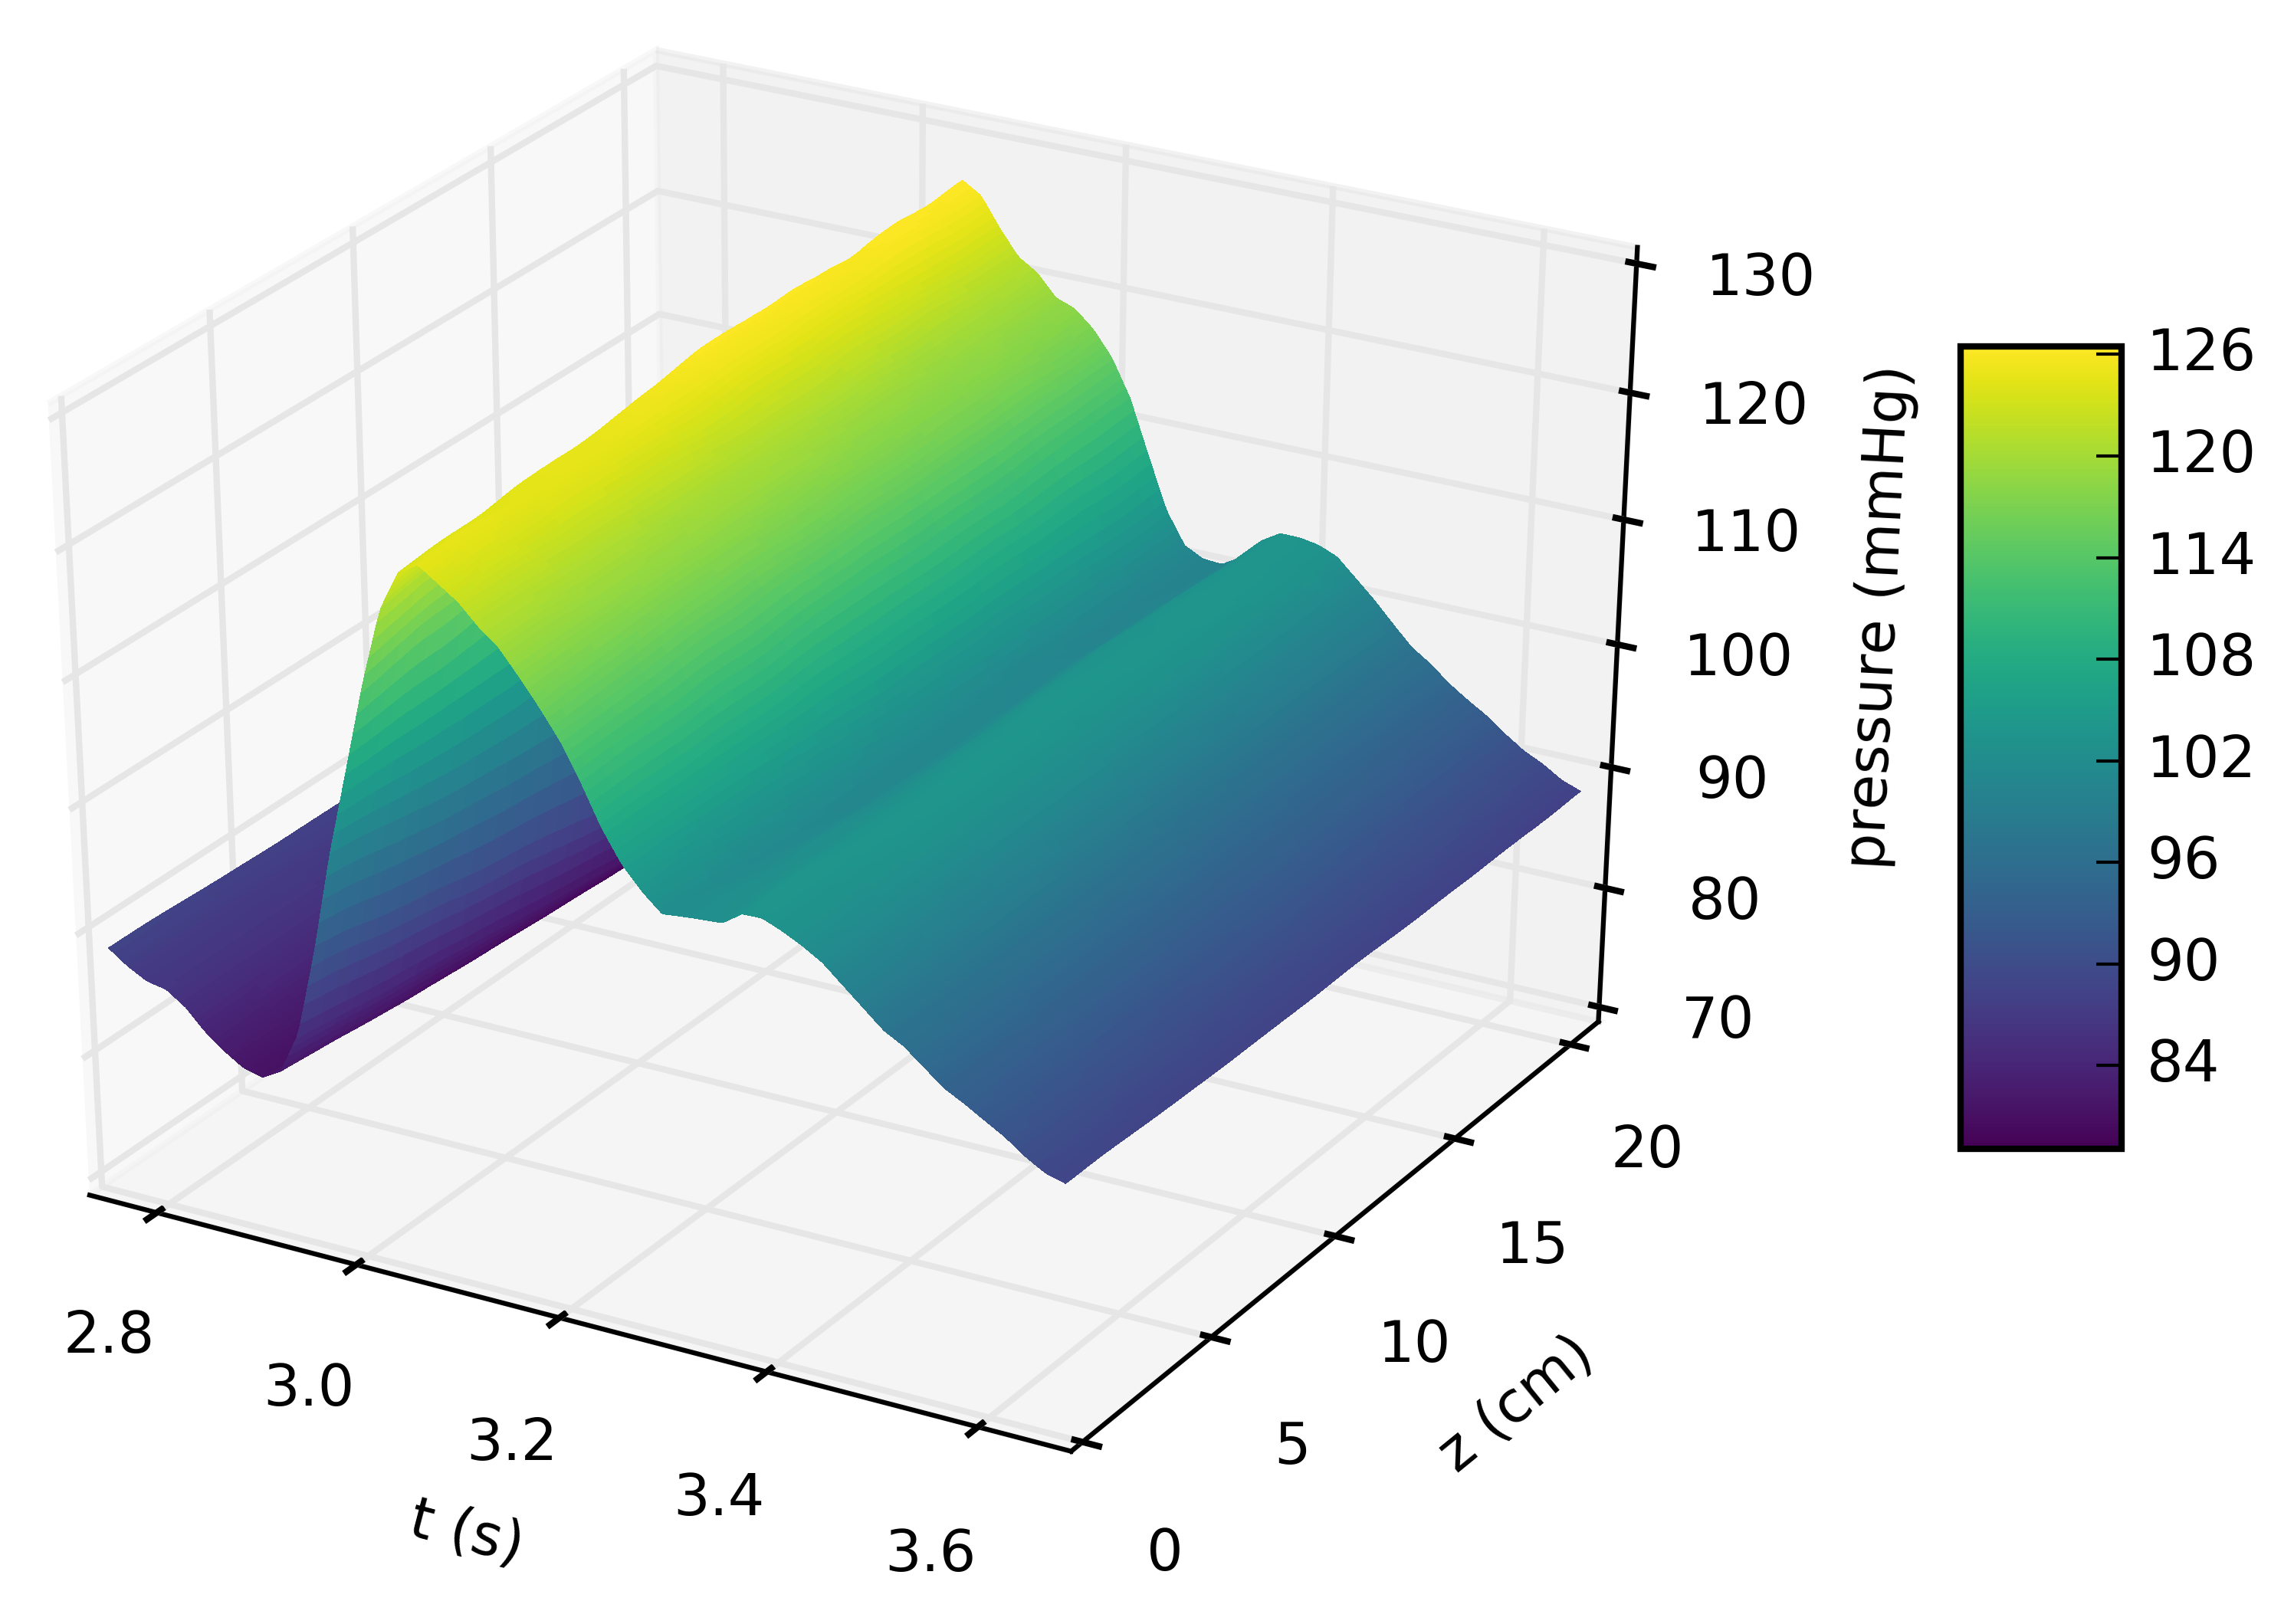
\includegraphics[width=\linewidth]{figure.png}
  \caption{A figure caption.\label{fig:1}}
\end{figure}

It references \fref{fig:1}.

\begin{table}
  \center
  \caption{A table caption.\label{tab:1}}
  \begin{tabular}{cc}
    \toprule
    Column 1 & Column 2\\
    \bottomrule
  \end{tabular}
\end{table}

It also references \tref{tab:1}.

\chapter{Another Chapter}
The text for another chapter goes here.

\begin{figure}
  \begin{algorithm}[caption={An algorithm caption.}, label=alg:1]
    i = 0
    while True:
      i += 1
  \end{algorithm}
\end{figure}

It references \aref{alg:1}.

You can also write inline code using

\begin{python}
i = 0
while True:
  i += 1
\end{python}

\appendix
\chapter{Appendix}
The text for an appendix goes here.

%% ----------------------------------------------------------------
\backmatter
%\bibliographystyle{plainnat}
%\bibliography{thesis}
\end{document}
%% ----------------------------------------------------------------
